%************************************************
\chapter{Introduction}\label{ch:introduction}
%************************************************
\section{Background and Context}
Autonomous systems are complex agents capable of carrying out operations without human intervention. They have become more capable thanks to technological advancements and increasingly integrated into society with recent remarkable progress in artificial intelligence (AI) techniques. According to Zhang in \cite{Zhang2017}, current trends indicate that the development and adoption of such systems will continue to grow in the coming years.

The agricultural sector is one of the areas where the integration of autonomous technologies has great potential. These systems could significantly benefit farmers by making their work safer and less repetitive. Autonomous systems have already been used in alternative cropping methods such as precision agriculture. Nevertheless, traditional practices are still facing challenges that autonomous systems could perfectly address. Among these challenges, the proliferation of weeds in grass fields raises as a major concern for the livestock well-being for two main reasons. First, weeds compete with grass for resources, causing forage loss \cite{Klotzli2024}. Second, some weed species pose a direct threat to livestock health. In particular, plants like Herbstzeitlose (Colchicum autumnale) have been identified as toxic and the cause of livestock poisoning \cite{Mueller2022}.

Removing these plants is a task that organic farmers must perform manually, as EU regulations restrict the use of pesticides and prevent farmers from combating weed proliferation through chemical means. It is evident that this task, especially in large grass fields, is highly time-consuming and extremely repetitive, making it an ideal candidate for automation. In Germany, companies like Paltech have developed solutions to address this problem using autonomous wheeled robots. Their flagship robot is a differential-drive wheeled system equipped with various sensors for localization and weed detection, as well as an onboard mechanism for weed removal. Currently, if the weed removal process needs to be sped up, the only solution is to deploy a fleet of robots. While this is feasible, developing single units capable of holding more than one weed control mechanism seems like the natural next step in Paltech's solution.

\section{Problem Definition}
% 1) What is the problem, why is it important? \\

The development of systems with more than one mechanism for weed removal comes with both hardware and software challenges. It is crucial to ensure that tools and system resources are used as efficiently as possible. Paltech wants to avoid having more capable units with unused tools, especially since the production and deployment of these improved systems are more costly. Therefore, reducing idle time is a top priority and the focus of this thesis.

% 2) What are the technology challenges, and, in particular, what are the overall areas that must be addressed to solve the technical aspects of the problem? \\

Idle time refers to periods when resources, such as tool equipment, are not actively engaged in productive work. Reducing idle time in this context means minimizing the time tools remain unused and maximizing their productivity in weed removal. To achieve this, allocating detected plants to the correct tools is essential. In the literature, this process is known as \ac{TA}. Some technical challenges to consider during implementation include computational latency and multi-tool coordination. The \ac{TA} algorithm and execution pipeline must be fast enough to process new detections and reassign tools in real time without causing delays, while also ensuring that multiple tool units operate efficiently without interference or redundancy.

\section{Related Work}
% 3) What are the capabilities of the current technology in the literature? \\

In general, a \ac{TA} system aims to achieve an efficient assignment of tasks to robots (or tools in this case) by considering various characteristics such as the robots' capabilities, task requirements, and system efficiency. This process of \ac{TA} involves three important factors to be consider acording to Umashankar in \cite{Umashankar2024}. Robot/tool, environment and coordination as shown in Figure \ref{fig:task-allocation-classification}.

\begin{figure}[bth]
    \centering
    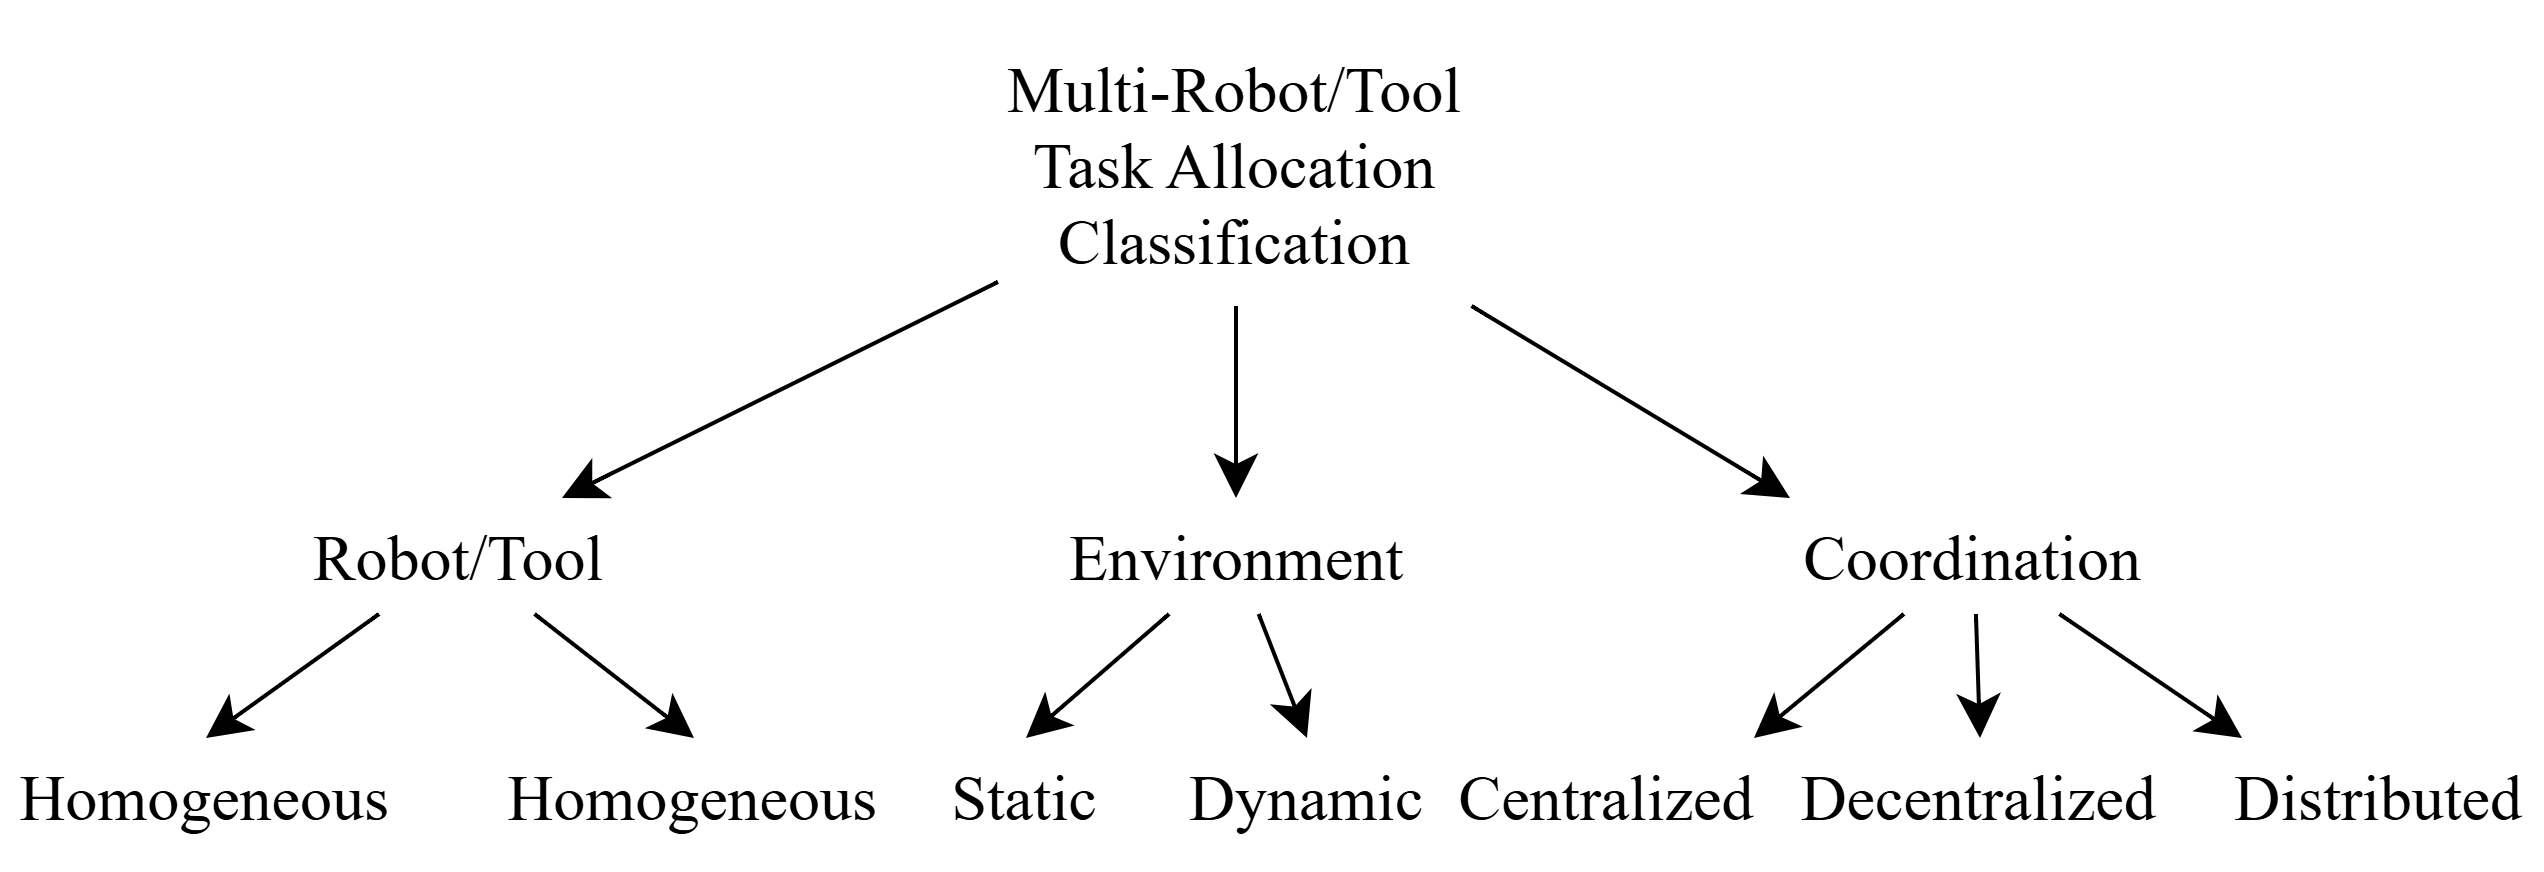
\includegraphics[width=0.9\linewidth]{gfx/ch01/task-allocation-classification.png}
    \caption{Task Allocation classification.}
    \label{fig:task-allocation-classification}
\end{figure}

An example of homogeneous tools in this context is a robot equipped with multiple tools of the same type, such as drills. In contrast, heterogeneous tools refer to robots equipped with different types of tools, such as drilling, seeding, and sensing equipment.

The multi-tool \ac{TA} can take place in either a dynamic or static environment. In an environment that is static in nature, tasks are allocated to tools in advance before they begin to execute them. This method works well in situations when the tasks are predetermined and the environment remains unchanged. In contrast, dynamic \ac{TA} involves the real-time assignment of tasks to tools as they carry out their activities. For the scope of this thesis, we will focus on homogeneous tools operating in a dynamic environment with centralized coordination, where the onboard computer will act as the master, assigning plants to each weed control mechanism.

There are several ways to accomplish multi-tool allocation, including heuristic, cluster-based, market-based, learning-based, and optimization-based techniques. Table \ref{tab:task-allocation-approaches-1} and \ref{tab:task-allocation-approaches-2} presents a comprehensive classification of \ac{TA} algorithms found in the literature \cite{Umashankar2024}.

\begin{table}[htbp]
    \myfloatalign
    \setlength{\tabcolsep}{1.5em} % Default is 0.5em
    \begin{tabularx}{\textwidth}{Xll}
        \toprule
        \tableheadline{Approach} & \tableheadline{Technique/Algorithm}                          \\
        \midrule

        \multirow{6}{*}{Cluster Based}
                                 & \acs{SVCA}\label{acro:SVCA}              \cite{Martin2023}   \\
                                 & Group Agent Partitioning                 \cite{Junyan2021}   \\
                                 & \acs{CBDTA}\label{acro:CBDTA}            \cite{Chen2018}     \\
                                 & \acs{VDKM}\label{acro:VDKM}              \cite{Kim2020}      \\
                                 & \acs{CBBA}\label{acro:CBBA}              \cite{Smith2014}    \\
                                 & K-Means Clustering                       \cite{Lu2018}       \\
        \midrule

        \multirow{7}{*}{Market Based}
                                 & Auction Algorithm                        \cite{Jiamei2022}   \\
                                 & Improved Auction Algorithm               \cite{Shiguang2021} \\
                                 & \acs{SSI}\label{acro:SSI} Auction Algorithm \cite{Dong2018}  \\
                                 & Extended \acs{SSI}                       \cite{Shi2021}      \\
                                 & Multihop-Based auction Algorithm         \cite{Lee2015}      \\
                                 & \acs{CBPAEA}\label{acro:CBPAEA}          \cite{Das2015}      \\
                                 & Distributed Auction-Based Algorithm      \cite{Luo2013}      \\
        \bottomrule
    \end{tabularx}
    \caption[Task Allocation approaches (1/2)]{Comparative overview of cluster-based and market-based approaches to Task Allocation.}
    \label{tab:task-allocation-approaches-1}
\end{table}

\begin{table}[thb]
    \myfloatalign
    \setlength{\tabcolsep}{2.5em} % Default is 0.5em
    \begin{tabularx}{\textwidth}{Xll}
        \toprule
        \tableheadline{Approach} & \tableheadline{Technique/Algorithm}                                         \\
        \midrule

        \multirow{6}{*}{Learning Based}
                                 & \acs{GRU}\label{acro:GRU}, \acs{MLP}\label{acro:MLP} \cite{Liu2022}         \\
                                 & Deep Reinforcement Learning                          \cite{Elfakharany2021} \\
                                 & Heterogeneous Graph Attention Network                \cite{Wang2022}        \\
                                 & Capsule Attention-Based Mechanism                    \cite{Paul2022}        \\
                                 & \acs{EDACAM}\label{acro:EDACAM}                      \cite{Park2022}        \\
                                 & \acf{GNN}\label{acro:GNN}                            \cite{Banfi2022}       \\
        \midrule

        \multirow{9}{*}{Optimization Based}
                                 & Mixed-Integer Quadratic Program                      \cite{Notomista2022}   \\
                                 & \acs{STADAA}\label{acro:STADAA}                      \cite{Lindsay2021}     \\
                                 & \ac{PSO}\label{acro:PSO}                             \cite{Li2020}          \\
                                 & Integer Programming                                  \cite{Velhal2022}      \\
                                 & \ac{MIQP}\label{acro:MIQP}                           \cite{Siddharth2021}   \\
                                 & \acf{GA}\label{acro:GA}                              \cite{Jose2016}        \\
                                 & \ac{COQP}\label{acro:COQP}                           \cite{Gennaro2019}     \\
                                 & Heuristic Based                                      \cite{Zhao2016}        \\
                                 & Fuzzy Optimization                                   \cite{Valero2023}      \\
        \bottomrule
    \end{tabularx}
    \caption[Task Allocation approaches (2/2)]{Comparative overview of learning-based and optimization-based approaches to Task Allocation.}
    \label{tab:task-allocation-approaches-2}
\end{table}

In cluster-based approaches, the goal is to group tasks into a predefined number of clusters. Instead of assigning a single task to each tool, the clustering approach allocates entire groups of tasks to them, reducing the number of individual task assignments and computational complexity. Clustering approaches aim to minimize travel distance and maximize task coverage by grouping tasks effectively. However, the optimal clustering of tasks still needs further exploration. Although these approaches simplify \ac{TA}, they struggle to handle dynamic changes in the environment.

An optimization-based strategy aims to select the best solution from a set of available options. These solutions are constrained by specific conditions, and the optimal one is determined based on the objective function. The objective function represents the system's ultimate goal. Some of the optimization algorithms have poor robustness to uncertainties therefore this approach is more suitable for solving well-defined and static problems focusing on theoretically optimal or near-optimal solutions. Additionally, optimization-based approaches require more computational power and are less adaptable to changing environments.

Market-based approaches effectively handle highly combinatorial optimization problems. In this method, an auctioneer informs agents about available tasks and requests bids. Each agent evaluates its capacity to complete the tasks and submits a bid accordingly. The auctioneer then assigns tasks to the agent with the most favorable bid. Generally, \ac{TA} using this approach minimizes travel time. While these methods are flexible and scalable, they may not always achieve a globally optimal solution.

Recent approaches to \ac{TA} incorporate deep learning techniques such as graph neural networks and graph convolutional networks. These types of \ac{TA} methods are commonly referred as learning-based approaches. Most learning-based approaches struggle to generalize to larger-scale problem scenarios beyond those used during training. This characteristic is especially important because real-world \ac{TA} problems frequently require modeling scenarios whose costs increase with the number of tasks and robots. Table \ref{tab:approaches-comparison} gives a comparison between all the approaches, Source \cite{Umashankar2024}.

% 4) What are the technical gaps that remain? \\

\begin{table}[H]
    \centering
    \begin{tblr}{
        width = \linewidth,
        colspec = {Q[50]Q[187]Q[254]Q[248]Q[194]},
        cell{2}{2} = {Silver,t},
        cell{2}{3} = {Silver,t},
        cell{2}{4} = {Silver,t},
        cell{2}{5} = {Silver,t},
        cell{3}{2} = {t},
        cell{3}{3} = {t},
        cell{3}{4} = {t},
        cell{3}{5} = {t},
        cell{4}{2} = {Silver,t},
        cell{4}{3} = {Silver,t},
        cell{4}{4} = {Silver,t},
        cell{4}{5} = {Silver,t},
        cell{5}{2} = {t},
        cell{5}{3} = {t},
        cell{5}{4} = {t},
        cell{5}{5} = {t},
        }
        & Clustering                            & Optimization                                                & Market                                             & Learning                                \\
        \rotatebox[origin=c]{90}{Advantage}   & Simplifies TA~and reduces complexity  & Provides optimal solutions, suited for static problems & Flexible, scalable, decentralized                        & Adaptable, learns, and improves over time     \\
        \rotatebox[origin=c]{90}{Limitation}  & May not account for dynamics well     & Computationally intensive, less adaptable                   & May not be global optima, needs effective bidding & Requires training, initially sub-optimal \\
        \rotatebox[origin=c]{90}{Best case}   & Logical tasks                         & Well-defined, static problems                               & Dynamic environments with varying tasks                  & Complex and uncertain environments            \\
        \rotatebox[origin=c]{90}{Future work} & Dynamic clustering, online adaptation & Hybrid models, real-time optimization                       & Adaptive market mechanisms, incentive models             & Transfer learning, meta-learning
    \end{tblr}
    \caption{Comparison between Task Allocation approaches}
    \label{tab:approaches-comparison}
\end{table}

\section{Proposed Solution}
% 5) What are the proposed solution approaches?
As Table \ref{tab:approaches-comparison} illustrates, algorithm selection must be carefully considered based on the application's nature to achieve optimal performance. In a grass field clearing application, the environment is highly dynamic, especially since weed detections occur while the system is in motion. Therefore, market-based approaches are well-suited to ensuring the system adapts effectively to such conditions. However, this solution might not be optimal.

Optimization-based solutions, on the other hand, are known for providing optimal results, but they are typically more suited for static problems. In our case, although the environment is dynamic, this approach is still worth exploring. Since tasks are continuously added and removed from the allocation problem, the computation time at this task density may not be a significant issue, making real-time optimization feasible.

A graph search approach is also proposed, which becomes particularly interesting if the problem can be translated into a graph representation. Using well-known algorithms such as \ac{DFS} \cite{Tarjan1972} or Dijkstra's \cite{Dijkstra1959} can help find the lowest-cost solution and achieve effective resource allocation, reducing both idle time and overall mission duration.

Lastly, clustering and learning-based approaches will be discarded. Clustering due to the challenges of dynamic clustering and the need for online adaptation. Although it offers the advantage of simplifying \ac{TA}, its benefits diminish in low to medium density scenarios. Learning-based approaches are excluded because of the required training phase and the difficulty of generalizing across environments with varying task densities.